% *********************************************************************
% © 2021–2024 Jeremy Sylvestre
%
% Permission is granted to copy, distribute and/or modify this document
% under the terms of the GNU Free Documentation License, Version 1.3 or
% any later version published by the Free Software Foundation; with no
% Invariant Sections, no Front-Cover Texts, and no Back-Cover Texts. A
% copy of the license is included in the appendix entitled “GNU Free
% Documentation License” that appears in the output document of this
% PreTeXt source code. All trademarks™ are the registered® marks of
% their respective owners.
%
% *********************************************************************

\newcommand*{\xmin}{-5}
\newcommand*{\xmax}{25}
\newcommand*{\ymin}{-10}
\newcommand*{\ymax}{110}

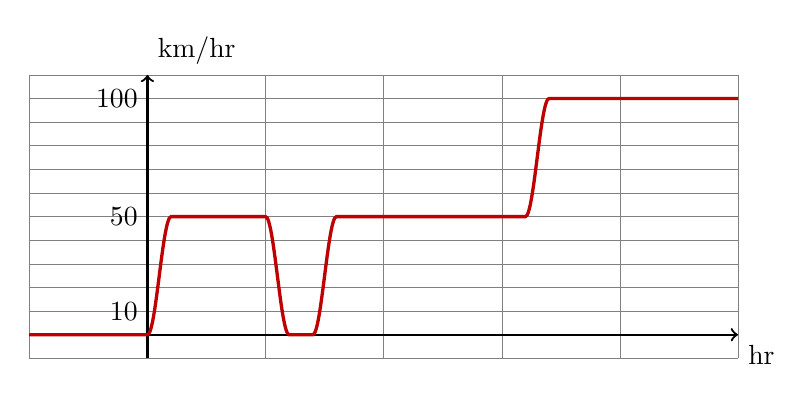
\begin{tikzpicture}
[
	closedpt/.style={circle,draw,fill,inner sep=0pt,minimum size=4pt},
	openpt/.style={circle,draw,inner sep=0pt,minimum size=4pt},
	xscale=0.3,
	yscale=0.03
]

	% grid
	\foreach \x in {-5,0,5,...,\xmax} {
		\draw[very thin,gray] (\x,\ymin) -- (\x,\ymax);
	}
	\foreach \y in {-10,0,10,...,\ymax} {
		\draw[very thin,gray] (\xmin,\y) -- (\xmax,\y);
	}

	% label grid
	% \node[below] at (6,0) {$0.1$};
	\foreach \y in {10,50,100} {
		\node[left] at (0,\y) {$\y$};
	}

	% axes
	\draw[->,thick] (\xmin,0) -- (\xmax,0) node[below right] {hr};
	\draw[->,thick] (0,\ymin) -- (0,\ymax) node[above right] {$\mathrm{km}/\mathrm{hr}$};

	% continuous graph
	\draw[red!75!black,very thick]
	  (\xmin,0) -- (0,0)
	  cos ( 0.5,  25)
	  sin ( 1,  50)
	  --  ( 5,  50)
	  cos ( 5.5,  25)
	  sin ( 6,   0)
	  --  ( 7,   0)
	  cos ( 7.5,  25)
	  sin ( 8,  50)
	  --  ( 16,  50)
	  cos ( 16.5,  75)
	  sin ( 17, 100)
	  --  ( 25, 100)
	;

\end{tikzpicture}
